\documentclass[11pt]{article}

% ---------- Packages ----------
\usepackage[margin=1in]{geometry}
\usepackage{amsmath, amssymb}
\usepackage{graphicx}
\usepackage{fancyhdr}
\usepackage{float}
\usepackage{listings}
\usepackage{xcolor}
\usepackage{cancel}
\usepackage[normalem]{ulem}

% ---------- MATLAB Code Listing Style ----------
\lstdefinestyle{matlab}{
    language=Matlab,
    basicstyle=\ttfamily\footnotesize,
    breaklines=true,
    breakatwhitespace=false,
    postbreak=\mbox{$\hookrightarrow$\space},
    columns=fullflexible,
    keepspaces=true,
    frame=none,
    numbers=left,
    numberstyle=\tiny,
    showstringspaces=false
}
\lstset{style=matlab}

% ---------- Paragraph Formatting ----------
\setlength{\parindent}{0pt}
\setlength{\parskip}{0.5em}

% ---------- Header ----------
\pagestyle{fancy}
\fancyhf{}
\lhead{ASEN 5335 Aerospace Environment}
\rhead{Justin Le}
\cfoot{\thepage}

% ---------- Document ----------
\begin{document}

% ---------- Title ----------
\begin{center}
    {\Large \textbf{Homework 4}}\\[0.5em]
    {\large ASEN 5335 Aerospace Environment}\\[0.5em]
    Justin Le\\ 
    \today
    \\[0.5em]
\end{center}

\vspace{1em}
\section*{Problem 1: Field Magnitudes}
% REFERENCES:
% - Module4 PDF p7-8, Sec 3.4 The Surface Field: WMM vs IGRF, definitions of F, I, D;
%   declination undefined at the poles because the field is vertical there
% - L14 slides 14, 16-19: F/I/D coordinates, declination map, inclination from H and Z
\hspace*{2em}Using the WMM model from the NOAA calculator, we find the magnetic 
field in Boulder, CO to be,
\begin{figure}[H]
    \centering
    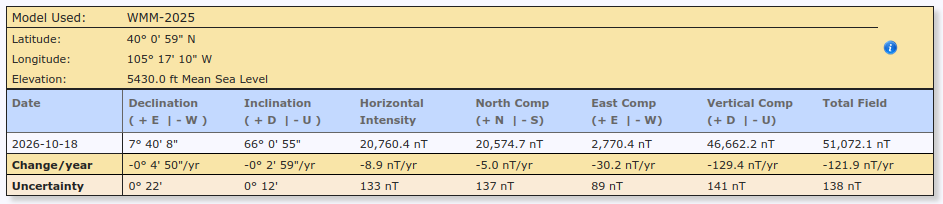
\includegraphics[width=1\textwidth]{Boulder_Magnetic_Field.png}
    \caption{Boulder Magnetic Field}
    \label{fig:Boulder_Magnetic_Field}
\end{figure}

\hspace*{2em}We repeat with the same model for McMurdo Station Anarctica to find,
\begin{figure}[H]
    \centering
    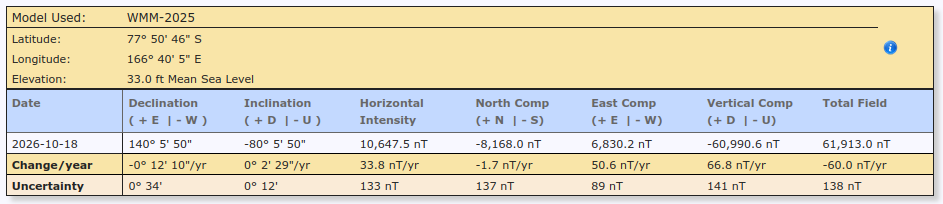
\includegraphics[width=1\textwidth]{McMurdo_Magnetic_Field.png}
    \caption{McMurdo Magnetic Field}
    \label{fig:McMurdo_Magnetic_Field}
\end{figure}

\hspace*{2em}\sout{Based on the inclination observed at McMurdo, this tells us that the magnetic fields will pass through the station based on the inclination and the latitude of the station.}

\hspace*{2em}\textcolor{red}{The inclination at McMurdo is about $-80^\circ$. This tells us that the magnetic field lines above McMurdo are
almost completely vertical, since the station is close to the magnetic pole.}

\newpage
\section*{Problem 2: Dipole Field}
% REFERENCES:
% - Module4 PDF p3, eqs (6)-(8): B_r, B_theta, |B| = B0 (RE/r)^3 sqrt(1 + 3 sin^2 lambda)
% - Module4 PDF p5, eq (11), Sec 3.2.1: field line equation r = L RE cos^2 lambda
% - L14 slide 21: annotated B-field components and magnitude, B0 ~ 31,000 nT
\subsection*{(i).}
\hspace*{2em}Assuming a dipole field model with $L=4$ $B_0 = 31,000~\mathrm{nT}$, $R_E = 6371~\mathrm{km}$, and at the equator ($\lambda=0^\circ$), we can use the following equations
to calculate the magnetic field magnitude,

\begin{gather*}
r = LR_E \cos^2 \lambda \\
|B| = B_{0} (\frac{R_E}{r})^3 \sqrt{1+3\sin^2\lambda}\\
\\
\therefore r = 25,484,000 \\
\boxed{\therefore |B| = 484.4~\mathrm{nT}}
\end{gather*}

\subsection*{(ii).}
\hspace*{2em}Repeating the above equations only for $\lambda = 30^\circ$,
\begin{gather*}
\therefore r = 19,113,000 \\
\boxed{\therefore |B| = 1518.9~\mathrm{nT}}
\end{gather*}

\newpage
\section*{Problem 3: Magnetopause}
% REFERENCES:
% - Module4 PDF p16-17, Sec 3.7.1, eq (34): rho v^2 = (2B)^2 / 2mu0 with B = B0/L^3;
%   factor of 2 comes from the magnetopause current
% - L16 slide 4: annotated standoff derivation, L ~ 10 for 5 /cm^3 and 400 km/s
% - L16 slide 24: "factor of two" note on IMF polarity slide
\subsection*{(i).}
\hspace*{2em}To find the standoff distance of the Earth to the magnetosphere,
we can use the equation, 

\begin{gather*}
\rho_{sw} v_{sw}^2 = \frac{(2B_{mag})^2}{2\mu_0} = \frac{4B_0^2}{2\mu_0 L^6} \\
B_{mag} = B_0 \left(\frac{R_E}{r}\right)^3 = \frac{B_0}{L^3}, \qquad B_0 \approx 31{,}000 \text{ nT} \\
L = \left(\frac{2B_0^2}{\mu_0 \rho_{sw} v_{sw}^2}\right)^{1/6}
\end{gather*}

\hspace*{2em}Given $v_{sw} = 400~\mathrm{km/s}$, and $\mu_0 = 4\pi \times 10^{-7}$, 
and $\rho_{sw} = nm_p = 5~\mathrm{proton/cm^3}*1.672\times10^{-27}~\mathrm{kg} = 8.36\times10^{-21}~\mathrm{kg/m^3}$.
\begin{gather*}
\boxed{L = 10.2}
\end{gather*}
\hspace*{2em}\textcolor{red}{Since we are above the equator, $L = 10.2$ gives a standoff distance of $10.2\,R_E$.}

\subsection*{(ii).}
\hspace*{2em}We can repeat the calculation above but instead using $v=1000~\mathrm{km/s}$, and $n=10~\mathrm{proton/cm^3}$, for a new $\rho_{sw} = 1.67\times10^{-20}~\mathrm{kg/m^3}$.
\begin{gather*}
\boxed{L = 6.7}
\end{gather*}
\hspace*{2em}\textcolor{red}{This gives a standoff distance of $6.7\,R_E$.}


\newpage
\section*{Problem 4: The Ring Current}
% REFERENCES:
% - Module4 PDF p15, eqs (32)-(33): gradient force and v_dgradB = (m v_perp^2 / 2q)(B x gradB)/B^3;
%   protons drift west, electrons east -> net westward current
% - Module4 PDF p16, Table 2: drift periods vs L and energy (sanity check, e.g. 100 keV
%   at L=3 is 2.44 h); notes relativistic electrons drift slower
% - Module4 PDF p19, Sec 3.7.4 The Ring Current; p26 states 85 keV average energy
% - L15 slides 19-20: gradient drift and drift period table
% - L16 slide 10: ring current, 3-6 RE, protons west / electrons east
% - Note: dipole at equator gives |gradB| = 3B/r (not stated explicitly, follows from B = B0/L^3)
\subsection*{(i).}
\hspace*{2em}The reason why there is a current in the first place is because of protons drifting west, while electrons drift east. This causes a net westward current which is the ring current. Additionally, drift speed scales with energy, this leads to the current being stronger where hotter particles (resulting in more energy) sitting at a higher altitude in the atmosphere at about 3-6 $R_E$.

\hspace*{2em}\textcolor{red}{The drift comes from the $\nabla B$ gradient drift (with some contribution from curvature drift), since $\nabla B$
points toward the Earth and $\bold{B}$ points up at the equator. The two key factors are a) the gradient drift moving the charged
particles around the Earth, and b) the drift direction depending on the charge. If ions and electrons drifted in the same direction,
like in $\bold{E}\times\bold{B}$ drift, there would be no net current.}

\subsection*{(ii).}
\hspace*{2em}Finding how long it takes for an $85~\mathrm{keV}$ electron to drift all the around Earth at $L=4$, we can use the equations, 
\begin{gather*}
\bold{v}_{d\nabla} = \frac{mv_{\perp}^2}{2q} \frac{\bold{B}\times \nabla B}{B^3} \\
E = \frac{1}{2}m v_{\perp}^2
\end{gather*}

\hspace*{2em}If we assume the particle remains in the equator and all its energy is perpendicular ($v_{\parallel} = 0$). At the equator $|\bold{B}\times\nabla B| = B|\nabla B|$. The drift speed is then,
\begin{gather*}
v_d = \frac{2E}{2q}\frac{B|\nabla B|}{B^3} = \frac{E}{qB}\frac{|\nabla B|}{B}
\end{gather*}

\hspace*{2em}To find the gradient we use the dipole field at the equator ($\lambda = 0^\circ$) from Problem 2 and take the derivative with respect to $r$,
\begin{gather*}
B = B_0\left(\frac{R_E}{r}\right)^3 \\
\frac{dB}{dr} = -3B_0\frac{R_E^3}{r^4} = -\frac{3B}{r} \\
\therefore |\nabla B| = \frac{3B}{r}
\end{gather*}

\hspace*{2em}Substituting the gradient back into the drift speed,
\begin{gather*}
v_d = \frac{E}{qB}\frac{3B}{rB} = \frac{3E}{qBr}, \qquad B=\frac{B_0}{L^3}, \quad r = LR_E
\end{gather*}

\hspace*{2em}The time to drift all the way around the Earth is the circumference of the drift path divided by the drift speed,
\begin{gather*}
T = \frac{2\pi r}{v_d} = \frac{2\pi qBr^2}{3E} = \frac{2\pi q B_0 R_E^2}{3EL}
\end{gather*}

\hspace*{2em}Given $L=4$, $B_0 = 31,000~\mathrm{nT}$, $R_E = 6371~\mathrm{km}$, and $E = 85~\mathrm{keV}$, we have $B = 484.4~\mathrm{nT}$ (from Problem 2) and $r = 25,484,000~\mathrm{m}$.
\begin{gather*}
v_d = \frac{3(85,000)}{(484.4\times10^{-9})(25,484,000)} = 20,660~\mathrm{m/s} \\
T = \frac{2\pi(25,484,000)}{20,660} = 7,750~\mathrm{s} \\
\boxed{\therefore T \approx 2.15~\mathrm{hours}}
\end{gather*}

\newpage
\section*{Problem 5: Drift due to Gravity}
% REFERENCES:
% - Module4 PDF p15, eq (31): v_dg = m g x B / (q B^2); drift direction and why the
%   proton term dominates (mass ratio)
% - Module4 PDF p13-14, eqs (28)-(29): general drift from any force, v_d = F x B / (q B^2)
% - L15 slide 16: "Third Motion: Particle Drifts"

\subsection*{(i.)}
\hspace*{2em}Under the influence of gravity, protons will drift east and electrons will drift west.
\subsection*{(ii.)}
\hspace*{2em}We find the magnitude of the drift velocity due to gravity is with the equation,
\begin{gather*}
\bold{v}_{dg} = \frac{m\bold{g}\times \bold{B}}{qB^2}
\end{gather*}
\hspace*{2em}\textcolor{red}{Using $g = 0.613~\mathrm{m/s^2}$ and $B = 484.4~\mathrm{nT}$ at $L=4$ (found in part (iii) and Problem 2), the magnitude for protons and electrons is,}
\begin{gather*}
\textcolor{red}{|v_{dg}| = \frac{mg}{|q|B}} \\
\textcolor{red}{|v_{dg}|_p = \frac{(1.673\times10^{-27})(0.613)}{(1.602\times10^{-19})(484.4\times10^{-9})}} \\
\boxed{\textcolor{red}{|v_{dg}|_p = 1.32\times10^{-2}~\mathrm{m/s}}} \\
\textcolor{red}{|v_{dg}|_e = \frac{(9.11\times10^{-31})(0.613)}{(1.602\times10^{-19})(484.4\times10^{-9})}} \\
\boxed{\textcolor{red}{|v_{dg}|_e = 7.20\times10^{-6}~\mathrm{m/s}}}
\end{gather*}
\hspace*{2em}\textcolor{red}{The mass in the numerator means electrons drift much slower than protons.}
\subsection*{(iii.)}
\hspace*{2em}To find how long it will take to drift around the Earth under gravity, we can use the drift due to gravity equation and assuming a particle drifting around the equator,

\begin{gather*}
\bold{v}_{dg} = \frac{m\bold{g}\times\bold{B}}{qB^2} \quad,~\quad v_{dg} = \frac{mg}{qB} \\
g = \frac{g_{Earth}}{L^2} = \frac{9.81}{4^2} = 0.613~\mathrm{m/s^2} \\
T = \frac{2\pi r}{v_{dg}} = \frac{2\pi qBr}{mg} \\
v_{dg} = \frac{(1.673\times10^{-27})(0.613)}{(1.602\times10^{-19})(484.4\times10^{-9})} = 1.32\times10^{-2}~\mathrm{m/s} \\
T = \frac{2\pi(25,484,000)}{1.32\times10^{-2}} = 1.21\times10^{10}~\mathrm{s} \\
\boxed{\therefore T \approx 384~\mathrm{years}} \\
\textcolor{red}{\text{This is for protons. For electrons,}} \\
\textcolor{red}{T_e = \frac{2\pi(25,484,000)}{7.20\times10^{-6}} = 2.22\times10^{13}~\mathrm{s}} \\
\boxed{\textcolor{red}{\therefore T_e \approx 705{,}000~\mathrm{years}}}
\end{gather*}

\hspace*{2em}Here we find that the drift due to gravity is far slower than the gradient drift from Problem 4, and that when calculating ring current this can be assumed to be a negligible effect. 

\newpage
\section*{Problem 6: Geomagnetic Indices}
% REFERENCES:
% - Module4 PDF p21-22, Sec 4.1: Kp / K / ap definitions; Kp ranges 0-9, each step
%   ~2x increase in magnetic activity
% - Rest is done on OMNIWeb (not covered in the notes)
\begin{figure}[H]
    \centering
    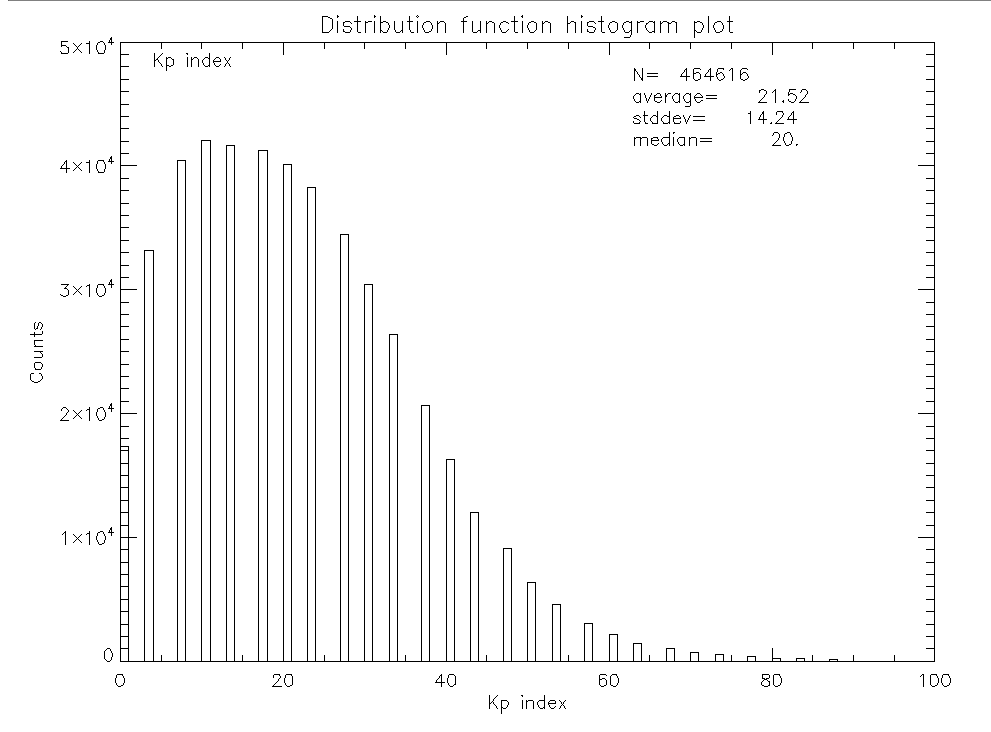
\includegraphics[width=0.8\textwidth]{Dist_function.png}
    \caption{Distribution Function}
    \label{fig:Dist_function}
\end{figure}

\subsection*{(i.)}
\hspace*{2em}Using Figure \ref{fig:Dist_function}, we can identify the most common Kp in this distribution as $Kp = 1$, as the most frequent occurrence in this distribution is at 10. 
\subsection*{(ii.)}
\hspace*{2em}Examining what values will be at level 9, we find the ratio of the Kp = 90 out of the total measurements. 
\begin{gather*}
\boxed{\frac{39}{464{,}616} = 0.0084\%}
\end{gather*}
\subsection*{(iii.)}
\hspace*{2em}When repeating the above for July 2004, we find,
\begin{figure}[H]
    \centering
    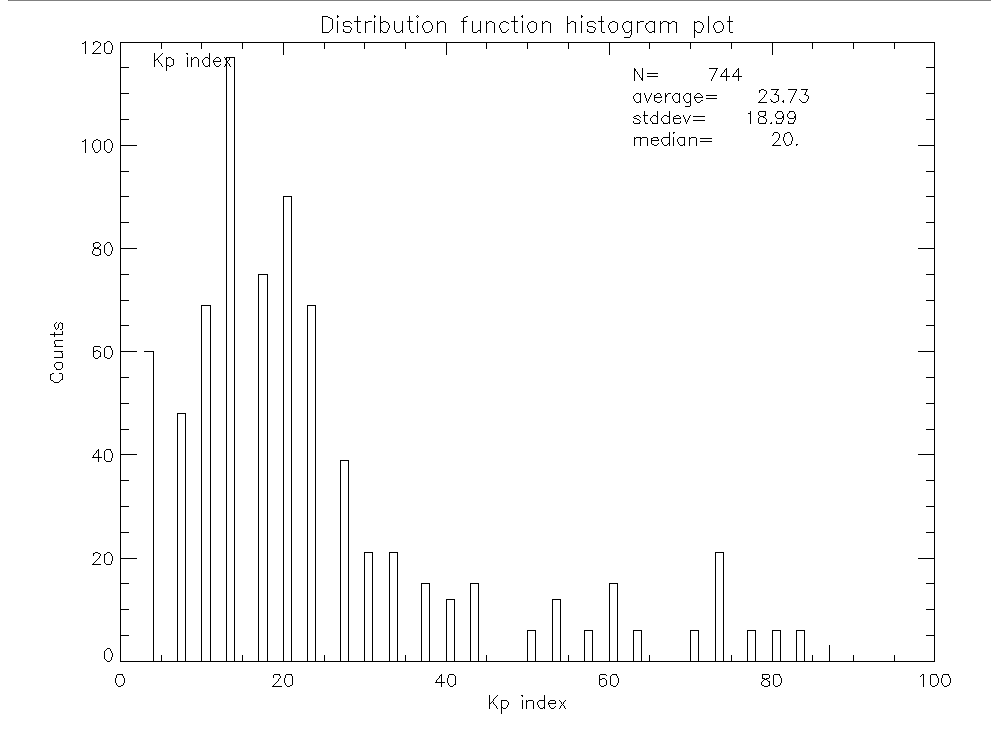
\includegraphics[width=0.8\textwidth]{Dist_function_iii.png}
    \caption{Distribution Function for July 2004}
    \label{fig:Dist_function_iii}
\end{figure}
Here we find that the most common Kp is \sout{11, so most common Kp is $Kp = 1.1$} \textcolor{red}{13, so most common Kp is $Kp = 1+$}, and there are no occurrences of Kp level 9.

\hspace*{2em}\textcolor{red}{Comparing the relative frequency of $Kp > 5$ (including $Kp = 5+$, $Kp*10 \geq 53$), July 2004 has}
\begin{gather*}
\textcolor{red}{\frac{87}{744} = 11.7\%} \\
\textcolor{red}{\text{while the 1964-2016 interval has}} \\
\textcolor{red}{\frac{14{,}514}{464{,}616} = 3.12\%}
\end{gather*}
\hspace*{2em}\textcolor{red}{July 2004 was more disturbed than typical.}

\newpage
\section*{Problem 7: Geomagnetic Storm}
% REFERENCES:
% - L16 slide 12: current loop dB = mu0 I / 2R (key equation for part ii)
% - Module4 PDF p2, eq (1): Biot-Savart law
% - Module4 PDF p21: why Dst is negative / measures the ring current; storm-level Dst thresholds
% - Module4 PDF p22: Halloween 2003 double storm
% - L16 slides 19-20: Dst station network and October 2003 Dst plot
\subsection*{(i.)}
\hspace*{2em}We can recreate the Halloween Storm and obtain the following,
\begin{figure}[H]
    \centering
    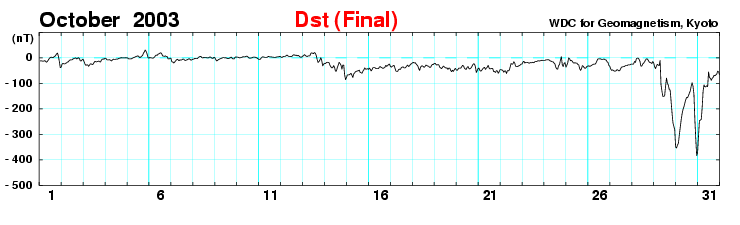
\includegraphics[width=0.8\textwidth]{dst200310.png}
    \caption{DST Index for the Halloween Storm}
    \label{fig:dst200310}
\end{figure}
\subsection*{(ii.)}
\hspace*{2em}Using this information, we can calculate the ring current magnitude with,
\begin{gather*}
B = \frac{\mu_0 I}{2R},~I = \frac{2RB}{\mu_0} \\
\mu_0 = 4\pi\times10^{-7}~\mathrm{Tm/A} \\
B = 400\times10^{-9}~\mathrm{T}\\
R = 5R_E = 5(6371)\times10^3~\mathrm{m}\\
\boxed{\therefore I = 20\times10^6~\mathrm{A}}
\end{gather*}

\newpage
\section*{Problem 8: Key Parameters in the Solar Wind Driving a Magnetic Storm}
% REFERENCES:
% - Module4 PDF p22, Sec 4.1.1 Storm Development: IMF Bz southward -> reconnection;
%   initial phase compression -> positive Dst
% - Module4 PDF p16 and L16 slide 5: magnetopause (Chapman-Ferraro) current, cause of the positive surge
% - Module4 PDF p20, Sec 3.7.6 Other Magnetospheric Currents
% - L16 slides 18, 24-25: storm progression, IMF polarity, reconnection
\subsection*{(i.)}
\hspace*{2em}The most critical parameter for describing solar wind is the interplanetary magnetic field. This is because for a geomagnetic storm to occur, the magnetic field field must point southward and also be sustained for an amount of time while also being stronger than usual, typically a result from coronal mass ejections. The interplanetary magnetic field essentially determines the conditions needed for a magnetic storm. \textcolor{red}{When the IMF is southward
with a large magnitude, it reconnects with Earth's dayside magnetic field, which transports more energy from the solar wind into the
magnetosphere and leads to the storm.}
\subsection*{(ii.)}
\hspace*{2em}The positive surge that results from the magnetopause current of the Chapman Ferraro current. This is because when a CME hits Earth, the higher solar wind pressure compresses the magnetosphere inward, which is the magnetic storm's initial phase. The current forms because the solar wind gyrating around the magnetopause field lines. This cancels out the Earth's field outside of the magnetosphere and increases the field inside of it, which leads to an eastward current as opposed to the usual westward current, causing a northward field and shows the surge in positive DST. 

\newpage
\section*{Problem 9: The Core}
% REFERENCES:
% - Module4 PDF p28-29, Sec 6 Movie: The Core (what's wrong with the premise)
% - Module4 PDF p1-2, Sec 3.1: field comes from the liquid OUTER core
% - L14 slides 10-11: core facts (inner core solid, Curie temperature, etc.)
% - Atmosphere module: why the atmosphere wouldn't "come apart"

\subsection*{(i.)}
\hspace*{2em}Aaron Eckhart's description of the Earth's core. His description is indeed accurate with a solid inner core and a swirling outer core. Physics 101, hot metal moving fast drives EM field, the hot metal swirling does indeed drive the EM field present on Earth, this can be seen in how its turbulent nature has previously led to the shifting and inverting. EM field does shield us from cosmic radiation, due to physics the EM field repels the cosmic radiation from Earth.

\subsection*{(ii.)}
\hspace*{2em}Microwave radiation will literally cook our planet, solar wind is not microwaves, and most of the radiation that would impact us would be absorbed by the atmosphere. Everybody on Earth is dead in a year, this is just a ridiculous timeline, the weakened field would not lead to extinction\textcolor{red}{, since even if the magnetic field turned off the atmosphere would continue to protect us from radiation}. Static discharges in the atmosphere will lead to superstorms, the EM field would have no impact on the weather effects seen in the lower parts of the atmosphere and the surface of Earth. \textcolor{red}{Static discharges in the atmosphere are lightning, which is a product of storms and does not cause them.}

\newpage
\section*{Problem 10: Magnetospheric Multiscale}
% REFERENCES:
% - Module4 PDF p28, Sec 5.2: mission objective (reconnection)
% - Parts ii-iv (spacecraft arrangement, instruments, orbit phases) not in the notes; use:
%   EO Portal: https://directory.eoportal.org/web/eoportal/satellite-missions/m/mms-observatory
%   NASA: https://mms.gsfc.nasa.gov
%   Paper: https://link.springer.com/article/10.1007/s11214-015-0164-9

\subsection*{(i.)}
\hspace*{2em}The primary objective of the MSS mission is to study the reconnection of magnetic field lines in Earth's magnetosphere. This is how the solar wind's magnetic field connects to Earth's and releases stored energy. It aims to look at small scale physics looking at how particles get accelerated and its turbulence. 
\subsection*{(ii.)}
\hspace*{2em}The reason why there were four spacecraft is because that allows for measuring data in 3D. They are arranged in a tetrahedron, where by taking 4 points of measurements not on the same plane, it allows measurements of 3 dimensions over time. 
\subsection*{(iii.)}
\hspace*{2em}All four spacecraft, carry the same instruments. The Hot Plasma Suite, which carry electron spectrometers (4 dual electron spectrometers, 4 dual ion spectrometers, and 1 HPCA), Energy Particle Detectors (2 FEEPS and 1 EIS), the FIELDS suite (4 spin-plane double probes, 2 axial double probes, 2 fluxgate magnetometers, 1 search coil magnetometer, and \sout{1 EDI} \textcolor{red}{2 EDI gun detector units (GDU)}), which was discussed in a previous homework, 2 ASPOC, which is the active spacecraft potential control to prevent the charge potential from building on the spacecraft. There are multiple instruments on each spacecraft because the spacecrafts rotate around its axis as spin stabilization keeps the spacecraft attitude steady without reaction wheels, resulting in sensors sweeping across the sky each rotation. \textcolor{red}{Spin stabilization also makes it possible to determine the full three-axis attitude instead of just the spin-axis direction.}

\subsection*{(iv.)}
\hspace*{2em}There are two phases in the mission, dayside and the magnetotail. They exist because there are two different conditions, in dayside the solar wind field lines will reconnect with Earth, at the magnetotail field lines stretched by solar storm reconnects. In dayside phase, the perigee would be $\approx 1.2 R_E$, the apogee is $\approx 12 R_E$. Meanwhile in the magnetotail phase the perigee is $\approx1.2 R_E$ but then the apogee is $\approx25 R_E$

\end{document}
